\documentclass[]{article}
\usepackage{lmodern}
\usepackage{amssymb,amsmath}
\usepackage{ifxetex,ifluatex}
\usepackage{fixltx2e} % provides \textsubscript
\ifnum 0\ifxetex 1\fi\ifluatex 1\fi=0 % if pdftex
  \usepackage[T1]{fontenc}
  \usepackage[utf8]{inputenc}
\else % if luatex or xelatex
  \ifxetex
    \usepackage{mathspec}
  \else
    \usepackage{fontspec}
  \fi
  \defaultfontfeatures{Ligatures=TeX,Scale=MatchLowercase}
\fi
% use upquote if available, for straight quotes in verbatim environments
\IfFileExists{upquote.sty}{\usepackage{upquote}}{}
% use microtype if available
\IfFileExists{microtype.sty}{%
\usepackage{microtype}
\UseMicrotypeSet[protrusion]{basicmath} % disable protrusion for tt fonts
}{}
\usepackage[margin=1in]{geometry}
\usepackage{hyperref}
\hypersetup{unicode=true,
            pdftitle={SOC2206\_Exercices revision},
            pdfauthor={Visseho Adjiwanou, PhD.},
            pdfborder={0 0 0},
            breaklinks=true}
\urlstyle{same}  % don't use monospace font for urls
\usepackage{longtable,booktabs}
\usepackage{graphicx,grffile}
\makeatletter
\def\maxwidth{\ifdim\Gin@nat@width>\linewidth\linewidth\else\Gin@nat@width\fi}
\def\maxheight{\ifdim\Gin@nat@height>\textheight\textheight\else\Gin@nat@height\fi}
\makeatother
% Scale images if necessary, so that they will not overflow the page
% margins by default, and it is still possible to overwrite the defaults
% using explicit options in \includegraphics[width, height, ...]{}
\setkeys{Gin}{width=\maxwidth,height=\maxheight,keepaspectratio}
\IfFileExists{parskip.sty}{%
\usepackage{parskip}
}{% else
\setlength{\parindent}{0pt}
\setlength{\parskip}{6pt plus 2pt minus 1pt}
}
\setlength{\emergencystretch}{3em}  % prevent overfull lines
\providecommand{\tightlist}{%
  \setlength{\itemsep}{0pt}\setlength{\parskip}{0pt}}
\setcounter{secnumdepth}{0}
% Redefines (sub)paragraphs to behave more like sections
\ifx\paragraph\undefined\else
\let\oldparagraph\paragraph
\renewcommand{\paragraph}[1]{\oldparagraph{#1}\mbox{}}
\fi
\ifx\subparagraph\undefined\else
\let\oldsubparagraph\subparagraph
\renewcommand{\subparagraph}[1]{\oldsubparagraph{#1}\mbox{}}
\fi

%%% Use protect on footnotes to avoid problems with footnotes in titles
\let\rmarkdownfootnote\footnote%
\def\footnote{\protect\rmarkdownfootnote}

%%% Change title format to be more compact
\usepackage{titling}

% Create subtitle command for use in maketitle
\newcommand{\subtitle}[1]{
  \posttitle{
    \begin{center}\large#1\end{center}
    }
}

\setlength{\droptitle}{-2em}

  \title{SOC2206\_Exercices revision}
    \pretitle{\vspace{\droptitle}\centering\huge}
  \posttitle{\par}
    \author{Visseho Adjiwanou, PhD.}
    \preauthor{\centering\large\emph}
  \postauthor{\par}
      \predate{\centering\large\emph}
  \postdate{\par}
    \date{12/5/2018}

\usepackage{float}

\begin{document}
\maketitle

\subsection{Exercice 1 : Type de
variables}\label{exercice-1-type-de-variables}

Parmi les exemples suivants, identifier les variables et dire si elles
constituent dans le contexte une variable dépendante ou indépendante.

\begin{enumerate}
\def\labelenumi{\arabic{enumi}.}
\item
  Une démographe analyse l'évolution du taux de fertilité des femmes
  depuis 1960 selon l'origine ethnique et le degré de scolarité.
\item
  Dans une expérience sur le temps de reeaction visuelle, on mesure le
  temps nécessaire pour percevoir des mots à connotation sexuelle par
  rapport à des mots non sexuels. Pour cette expérience, les chercheurs
  prennent bien soin de s'assurer que la vision des sujets leur permet
  de voir adéquatemment les diaspositives.
\item
  Un criminologue recherche des données sur la nature des infractions au
  Code criminel selon le sexe des accusés.
\item
  Lors d'une série d'expérience en psychologie sportive, on s'est rendu
  compte que chez les athlètes masculins, en situation de compétition
  relativement à celle de non compétition, il y a une augmentation du
  nombre de comportements complexes émis, mais qu'il y a une
  augmentation du nombre de comportements complexes émis, mais qu'il y a
  une baisse de la qualité de ceux-ci.
\item
  Des élèves du cours de psychologie expérimentale veulent étudier les
  sentiments de culbabilité des individus selon le type de délit qu'ils
  ont commis.
\item
  Un journaliste fait l'examen du pourcentage des intentions de vote des
  différents partis politiques québecois selon la langue parlée à la
  maison, le groupe d'âge et le degré de scolarité des électeurs.
\end{enumerate}

\subsection{Exercice 2 : Analyse
univariée}\label{exercice-2-analyse-univariee}

On a demandé à 4 ménages le revenu des deux conjoints, et le nombre de
personnes du ménage :

\begin{itemize}
\item
  conjoint1 \textless{}- c(1200, 1180, 1750, 2100)
\item
  conjoint2 \textless{}- c(1450, 1870, 1690, 0)
\item
  nb\_personnes \textless{}- c(4, 2, 3, 2)
\end{itemize}

Utiliser une calculatrice, ou R pour calculer:

\begin{enumerate}
\def\labelenumi{\arabic{enumi}.}
\item
  Le revenu total de chaque ménage
\item
  Le revenu moyen de chaque ménage
\item
  Le revenu par personne de chaque ménage
\item
  Quel indicateur vous semble le plus approprié pour exprimer le revenu
  du ménage?
\end{enumerate}

\subsection{Exercice 3 : Analyse
bivariée}\label{exercice-3-analyse-bivariee}

Dans ce qui suit on utilisera la base de données issue du recensement de
la population de 2012. Ces données contiennent les résultats partiels
concernant les communes de plus de 2000 habitants de France
métropolitaine et limitées aux données de 5 départements (``Oise'',
``Rhône'', ``Hauts-de-Seine'', ``Lozère'',``Bouches-du-Rhône''). Le
graphique suivant présente un résultat issu de ces données.

\begin{figure}
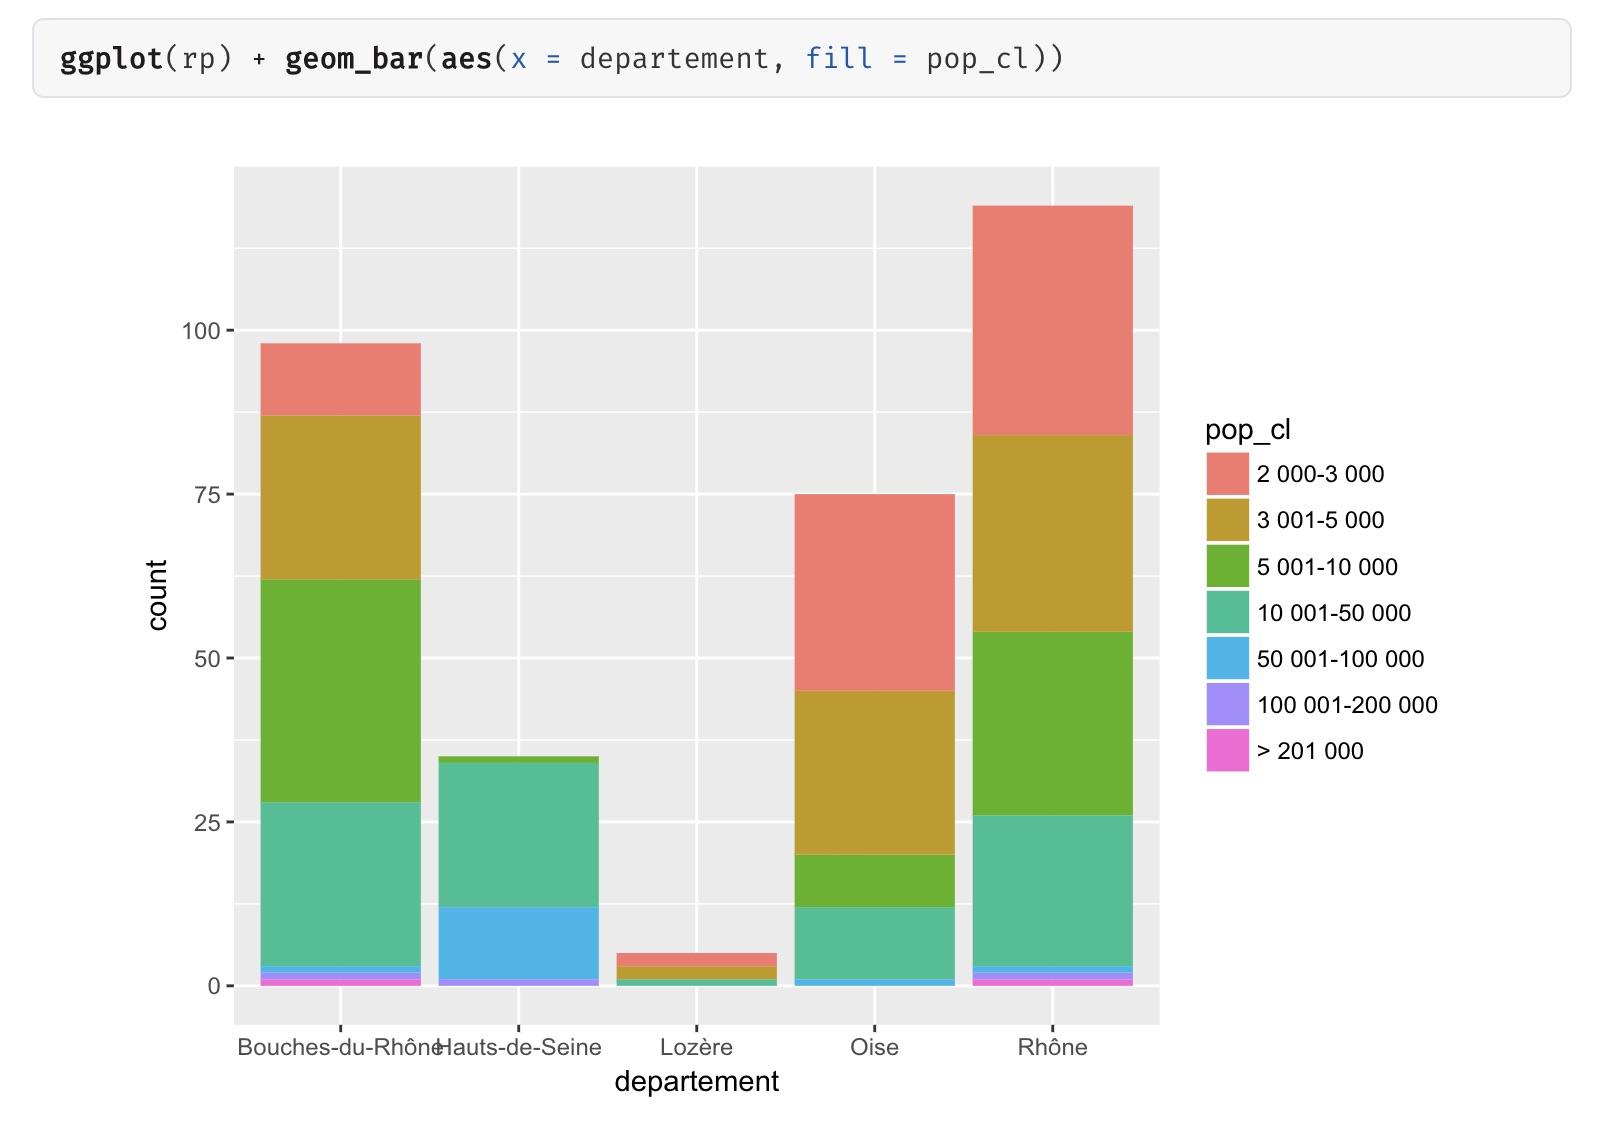
\includegraphics[width=1\linewidth]{Graphique1} \caption{Figure 1}\label{fig:pressure}
\end{figure}

\begin{enumerate}
\def\labelenumi{\arabic{enumi}.}
\item
  Que tente de faire ce graphique?
\item
  Interprétez les résultats de ce graphique.
\end{enumerate}

\subsection{Exercice 4 : Analyse
bivariée}\label{exercice-4-analyse-bivariee}

Une équipe d'étudiants choisit d'étudier, à l'intérieur d'un cours de
psychologie, le comportement des automobilistes hommes et femmes. Étant
donné la variété de comportements étudiables, l'équipe décide d'en
retenir quelques-uns qui puissent être observés aisément dans un temps
limité. Ils s'installent donc à une intersection où les automobilistes
doivent faire un arrêt. Ils notent le sexe de l'automobiliste et sa
réaction face au signal d'arrêt: il s'arrête complètement, il ne fait
que ralentir plus ou moins fermement ou bien, il ne fait pas d'arrêt et
passe tout droit.

Le tableau ci-dessous présente les résultats obtenus par l'équipe lors
d'un après-midi d'observation.

\begin{enumerate}
\def\labelenumi{\arabic{enumi}.}
\item
  Trouver la valeur des lettres A, B et C
\item
  Quelle est la population étudiée
\item
  Pour chaque variable, quel est le type d'échelle de mesure utilisé?
  Est-il toujours aisé de les appliquer dans le contexte de l'étude?
  Sinon, préciser quel type de difficultés est à envisager et comment il
  est possible d'y remédier.
\item
  Globalement, quelles proportions des automobilistes adoptent l'un des
  trois comportements observés?
\item
  Étant donné que c'est le comportement des hommes et femmes au volant
  que l'équipe veut étudier, laquelle des transformations en fréquences
  relatives l'équipe doit-elle appliquer sur le tableau de contingence
  qui a été dressé? L'appliquer et interpréter le résultat.
\item
  Comment présenterez-vous ce résultat dans un graphique? (Présenter le
  à partir de R, ne fera pas partie de l'examen)
\end{enumerate}

Tableau 1:Types de comportements enrégistrés aux signaux d'arrêt selon
le sexe des automobiles

\begin{longtable}[]{@{}lcrrr@{}}
\toprule
\textbf{Sexe} & Arrêt complet & Ralentissement & Pas d'arrêt &
\textbf{Total}\tabularnewline
\midrule
\endhead
Masculin & 41 & 39 & 15 & 95\tabularnewline
Féminin & 48 & 29 & 8 & 85\tabularnewline
\textbf{Total} & A & B & C & 180\tabularnewline
\bottomrule
\end{longtable}

\subsection{Exercice 5:
Échantillonnage}\label{exercice-5-echantillonnage}

L'insomnie est un problème très répandu. Diverse études épidémiologiques
démontrent qu'entre 15\% et 30\% de la population souffre d'insomnie.
Ces recherches indiquent également que l'insomnie augmente avec l'âge et
qu'elle est plus fréquene chez femmes. Compte tenu de ces informations,
vous désirez procéder à une enquête auprès d'un échantillon de la
population québécoise adulte afin de connaître les habitudes de sommeil
de cette population.

\begin{enumerate}
\def\labelenumi{\arabic{enumi}.}
\item
  Quelle serait votre population cible?
\item
  Quelle serait la meilleure méthode d'échantillonnage?
\item
  Discuter.
\end{enumerate}

\subsection{Exercice 6:
Échantillonnage}\label{exercice-6-echantillonnage}

\begin{enumerate}
\def\labelenumi{\arabic{enumi}.}
\item
  Vous désirez tirer un échantillon de taille 3 dans une population de
  taille 7. Combien de possibilité vous avez?
\item
  Voici une population U = \{A, B, C, D\}
\end{enumerate}

\begin{itemize}
\tightlist
\item
  Énumérer l'ensemble des échantillons de tailles 2 que vous pouvez
  tirer de cette population
\item
  Choisissez un échantillon parmi ceux-ci et calculer sa moyenne si A =
  1, B = 3, C = 5 et D = 2.
\item
  Est-ce que cette moyenne est semblable a la moyenne de la population?
\end{itemize}

\subsection{Exercice 7:
Échantillonnage}\label{exercice-7-echantillonnage}

De nombreuses études utilisent des mesures autodéclarées de
l'utilisation du téléphone mobile. C'est un cadre intéressant dans
lequel les chercheurs peuvent comparer le comportement autodéclaré avec
le comportement journalisé. Deux comportements communs à poser sont
l'appel et le texto, et deux trames communes sont ``hier'' et ``la
semaine dernière''.

\begin{itemize}
\tightlist
\item
  Q1: ``Combien de fois avez-vous utilisé votre téléphone portable pour
  appeler les autres hier?''
\item
  Q2: ``Combien de SMS avez-vous envoyé hier?''
\item
  Q3: ``Combien de fois avez-vous utilisé votre téléphone portable pour
  appeler les autres au cours des sept derniers jours?''
\item
  Q4: ``Combien de fois avez-vous utilisé votre téléphone mobile pour
  envoyer ou recevoir des SMS / SMS au cours des sept derniers jours?''
\end{itemize}

\begin{enumerate}
\def\labelenumi{\arabic{enumi}.}
\tightlist
\item
  Laquelle des mesures d'auto-évaluation est la plus exacte? Pourquoi?
\item
  Quelle meilleure approche utiliserez-vous pour recueillir ces
  informations? Quelles sont les limites de chaque approche?
\end{enumerate}

\subsection{Exercice 8: Causalité}\label{exercice-8-causalite}

Le tableau suivant vous donne le revenu moyen d'avant et d'après
l'introduction d'un programme de microfinance en Afrique du Sud entre
les participants (\textbf{groupe d'intervention}) et les
non-participants (\textbf{groupe de contrôle}) au programme :

\begin{figure}[H]
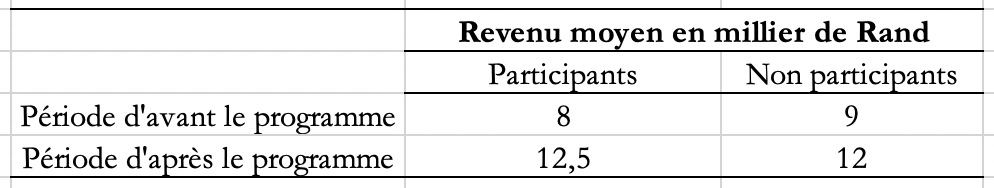
\includegraphics[width=0.9\linewidth]{Tableau1} \caption{Tableau 1}\label{fig:global_options}
\end{figure}

\begin{enumerate}
\def\labelenumi{\arabic{enumi}.}
\item
  Quelle est la différence moyenne de revenu mensuel du ménage entre le
  groupe d'intervention et le groupe de contrôle à la période d'apreès
  le programme? Cette différence est appelée comparaison transversale (.
\item
  Quelle est la différence moyenne entre le revenu mensuel du ménage
  avant et après l'intervention du groupe d'intervention ? Cette
  différence est appelée différence avant-après.
\item
  Quelles approche vous semble la plus appropriée pour mesurer l'effet
  du programme de microfinance?
\item
  Quelles sont les limites de chaque approche?
\item
  Comment pensez-vous combiner les deux approches pour une meilleure
  estimation de l'effet du programme?
\end{enumerate}

\subsection{Exercice 9: Régression
lineaire}\label{exercice-9-regression-lineaire}


\end{document}
